\section{k-nearest Neighbor}
From the beginning of the course we only have used linear methods. the issue about them is that a lot of the data in our world cannot be described as a linear model, take for instance this dataset:
\begin{center}
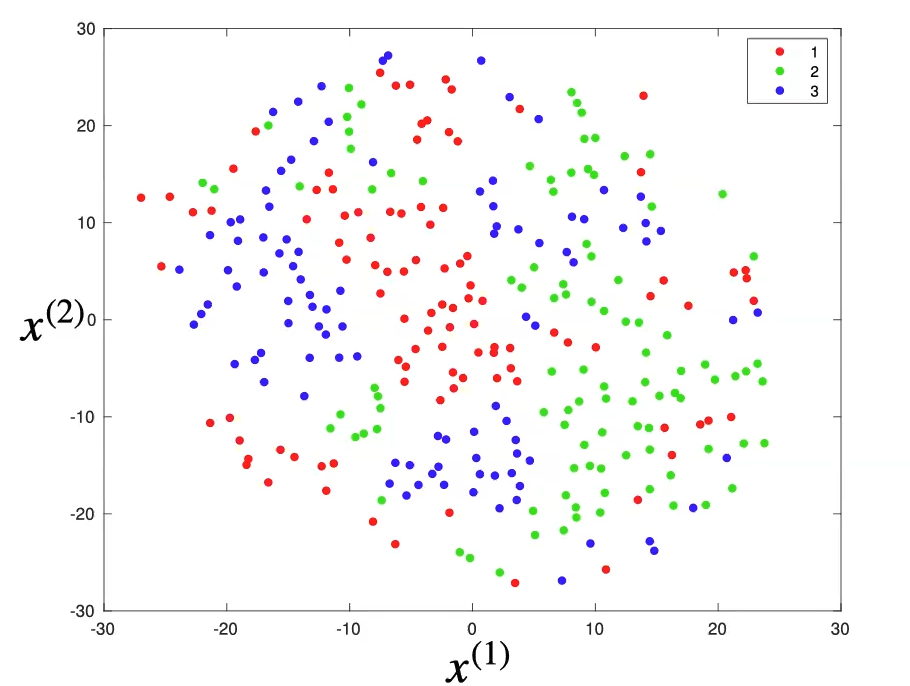
\includegraphics[scale=0.3]{screenshots/2026-03-10.png}
\end{center}
You cannot fit a linear model directly to this data. 

\begin{parag}{Intuition behind the nearest neighbor method}
    The intuition is that similar data samples have the same label. For instance if we take Maya glyph recognition (Hu et al., 2017) given a test sample, we look at the training sample that look a lot like the input sample and output the same ouput. This works with regression and classification.
\end{parag}

\subsection{NN: Algorithm}
The algorithm can be computed as follow:
\begin{enumerate}
    \item  Compute the distance between the test sample $x$ and all training samples $\left\{x_i\right\}$
    \item Find the sample $x_{NN}$ with minimum distance
    \item Assin the corresponding label/value $y_{NN}$ to the test sample
\end{enumerate}
\begin{center}
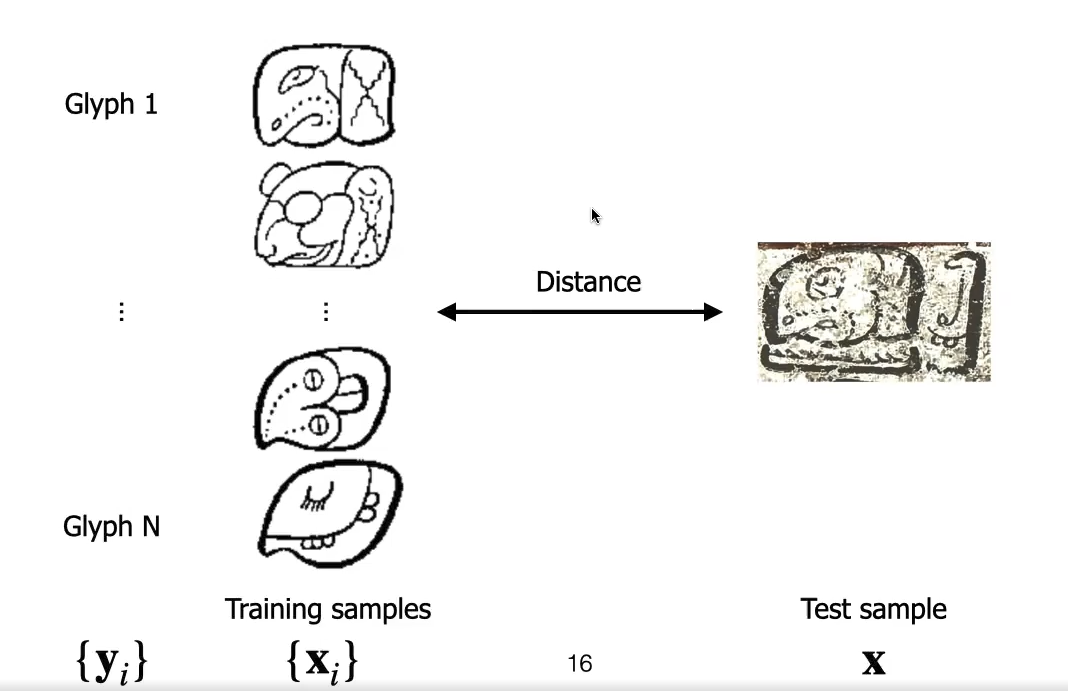
\includegraphics[scale=0.3]{screenshots/2026-03-10_1.png}
\end{center}
And this is our first \important{non-linear} algorithm!! In this case as in the linear model the results may change for different distance functions.

\begin{parag}{Example}
    Let us see a toy example with 3D histograms belonging to 2 classes (colors):
	\begin{center}
	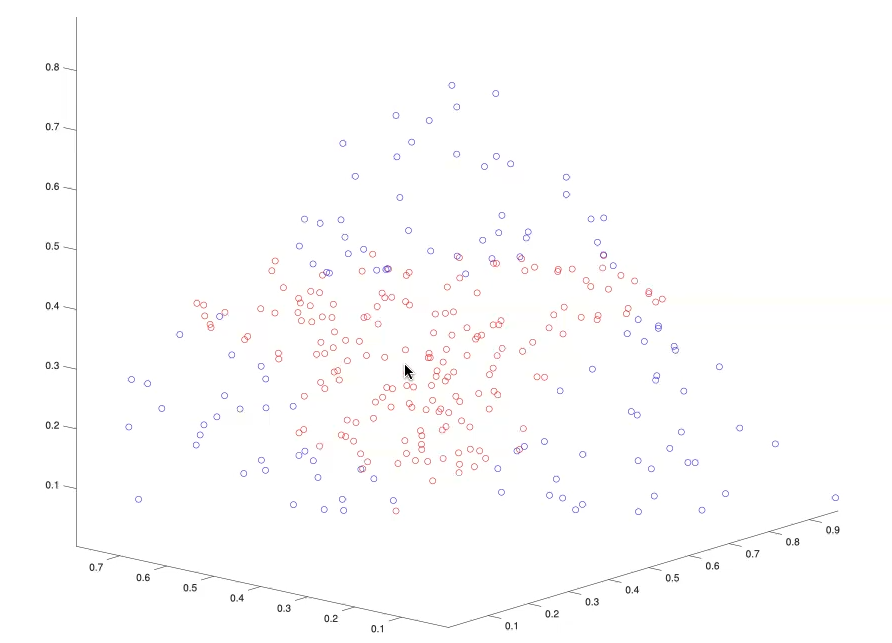
\includegraphics[scale=0.3]{screenshots/2026-03-10_2.png}
	\end{center}
\end{parag}
\paragraph{Histograms}%
\label{par:Histograms}
\begin{definition}
A \important{histogram} in $\mathbb{R}^{D}$ is a $D$-dimensional vector such that:
\begin{align*} 
	x^{\left(d\right)} \in [0, 1], \forall 1\leq d \leq D\\
	\sum_{d = 1}^{D} x^{\left(d\right)} = 1
\end{align*}
Given a vector $\mathbb{R}^{D}$ whose values are all non-negative (and at least one is stricly positive), one can obtain a histogram by dividing each value by the sum of values (normalize).
\end{definition}

\begin{parag}{Example}
    Let the original vector in $\mathbb{R}^{9}$ be:
	\begin{align*} 
		\widetilde{x} =  \begin{pmatrix} 1 & 2 & 1 & 2 & 1 & 1 & 0 & 0 & 0 \end{pmatrix}^{T}
	\end{align*}
	The sum of its value is:
	\begin{align*} 
		\sum_{d= 1}^{D} \widetilde{x}^{\left(d\right)} = 8
	\end{align*}
	Then, the histogram can be computed as:
	\begin{align*} 
		x = \begin{pmatrix} \frac{1}{8} & \frac{1}{4} & \frac{1}{8} & \frac{1}{4} & \frac{1}{8} & \frac{1}{8} & 0 & 0 & 0 \end{pmatrix} 
	\end{align*}
\end{parag}
intristingly, histograms live in a $D - 1$ dimension space, for instance if we take $n = 100$ samples in dimension $D = 2$ then our histogram can be:
\begin{center}
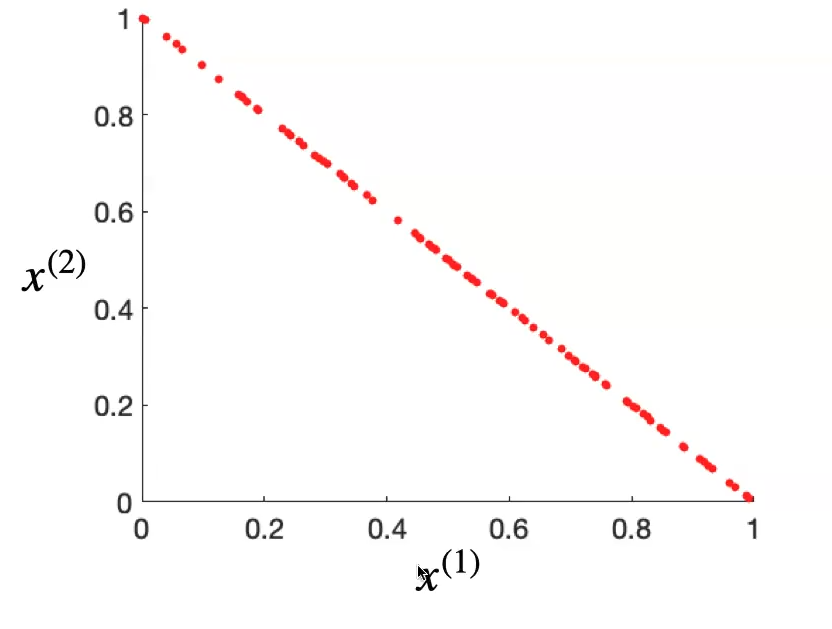
\includegraphics[scale=0.3]{screenshots/2026-03-10_3.png}
\end{center}

\begin{parag}{Back to NN}
    The default distance that we will use in our algorithm will be the euclidean distance:
	\begin{align*} 
		d\left(x_i,x\right) = \sqrt{\sum_{d = 1}^{D}\left(x_i^{\left(d\right)} - x^{\left(d\right)}\right)^2}
	\end{align*}
	Another fairly common used distance is the \important{Chi-square} distance:
	\begin{align*} 
		d\left(x_i, x\right) = \sqrt{\mathcal{X}^2\left(x_i, x\right)} = \sqrt{\sum_{d = 1}^{D}\frac{\left(x_i^{\left(d\right)} - x^{\left(d\right)}\right)^2}{x_i^{\left(d\right)} + x^{\left(d\right)}}}
	\end{align*}
	Another properties of the nn algorithm is that our results may be sensitive to outliers
	\begin{itemize}
	    \item A point close to the outlier (blue circle in the center) will be missclassified
	    \item Solution: Look at multiple neighbors instead of just one
	\end{itemize}
	This is the idea behind the k-nearest algorithm. Instead of taking only the nearest, we take $k$ nearest.
	
\end{parag}


\subsection{k-nearest neighbors}
The classification can be done as follow:
\begin{parag}{classification}

\begin{enumerate}
    \item Compute the distance between the test sample $x$ and all training samples $\left\{x_i\right\}$
    \item Find the $k$ samples $\left\{x_{NN1}, x_{NN2}, \ldots, x_{NNk}\right\}$ with minimum distances
    \item Find the most common label among these $k$ nearest neighbors (majority vote)
    \item Assign the corresponding label $y_{MV}$ to the test sample
\end{enumerate}
If severel labels appear the same number of times among the $k-NN$, one strategy consists of taking the one whose samples have the smallest average distance to the test sample.

\end{parag}
\begin{parag}{Regression}
    
\begin{enumerate}
    \item Compute the distance between the test sample $x$ and all training samples $\left\{x_i\right\}$
    \item Find the $k$ samples $\left\{x_{NN1}, x_{NN2}, \ldots, x_{NNk}\right\}$ with minimum distances
    \item Compute the value $\hat{y}$ for the test sample based on that of these $k-NN$
\end{enumerate}
	But how do we compute $\hat{y}$?
\end{parag}
\begin{parag}{Two strategies}
    Intuitively we can either choose two things two in order to compute the label:
	\begin{enumerate}
	    \item The number of label for each
	    \item The distance for each label
	\end{enumerate}
	Using the average of the $k-NN$ values $\left\{x_{NNi}\right\}$:
	\begin{align*} 
		\hat{y} = \frac{1}{k} \sum_{i= 1}^{k} y_{NNi}
	\end{align*}
	Using a weighted average of the $k-NN$ values, based on the inverse distances:
	\begin{align*} 
		\hat{y} = \frac{1}{\sum_{i= 1}^{k}w_{NNi}} \sum_{i= 1}^{k}w_{NNi}y_{NNi}
	\end{align*}
	Where
	\begin{align*} 
		w_{NNi} = \frac{1}{d\left(x_{NNi}, x\right)}
	\end{align*}
\end{parag}
\begin{framedremark}
To have a better visualization, we can use the demo here:
\href{http://vision.stanford.edu/teaching/cs231n-demos/knn/}{http://vision.stanford.edu/teaching/cs231n-demos/knn/}
\end{framedremark}
\begin{parag}{k-nearest: Example}
    What about performance, if we take the MNIST classification (which has 10'000 data sampes) for each of our methods we have:
\end{parag}
	\begin{center}
	\begin{tabular}{|c|c|c|c|}
		\hline
		Method & Preprocessing & Error in \% & Reference \\
		\hline
		K-nearest-neighbors, Euclidean ($L_2$) & none & 5.0 & LeCun et al.1998 \\
		\hline
		K-nearest-neighbors, Euclidean ($L_2$) & none & 3.09 & Kennet Wilder. U. Chicago \\
		\hline 
		K-nearest-neighbors, $L_3$ & none & 2.83 & Kenneth Wilder. U. Chicago \\
		\hline 
	\end{tabular}
	\end{center}
	If now we use preprocessing before using our algorithm defined above we can get:

	\begin{center}
	\begin{tabular}{|c|c|c|c|}
		\hline
		Method & Preprocessing & Error in \% & Reference \\
		\hline
		K-NN-neighbors, $L_2$ & deskewing & 2.4 & LeCun et al.1998 \\
		\hline
		K-NN-neighbors,  $L_2$ & deskewing, noise removal, blurring & 1.80 & Kennet U. Chicago \\
		\hline 
		K-NNneighbors, $L_3$ & deskewing, noise rem., blurring & 1.73 & Kenneth U. Chicago \\
		\hline 
		K-NN-neighbors, $L_3$ & deskewing, noise rem., blurring, 1 pixel shift & 1.33 & Kenneth U. Chicago \\
		\hline 
		K-NN-neighbors, $L_3$ & deskewing, noise rem., blurring, 2 pixel shift & 1.22 & Kenneth U. Chicago \\
		\hline 
	\end{tabular}
	\end{center}
	
	Using even fancier preprocessing (shiftable edges, subsampling to 16x16 pixels etc...) we can get up to 0.52 \% error.
	\begin{framedremark}
	Remember to put the face completion example
	\end{framedremark}
	\begin{parag}{k-nearest neighbors: Propeties}
	    There is no \important{learning} what we need is:
		\begin{itemize}
			\item a good data representation
			\item a distance function
			\item a given value $k$
		\end{itemize}
		This is referred to as a \important{non-parametric} learning method:
		\begin{itemize}
		    \item No parameters to optimize during training
		    \item $k$ is said to be a \important{hyper-parameter}, set manually (or by validation, which we will discuss in future lecture)
		\end{itemize}
		As we have seen before, k-nn can be a very good a predicting but there is always a downside, it is \important{computationally expensive}. For \important{each test sample}, one need to compute the distances to \important{all training samples}. There is solution for this where we approcimate nearest neighbor search:
		\begin{itemize}
		    \item Hashing
		    \item kd-trees
		\end{itemize}
	\end{parag}
	\begin{parag}{Curse of dimensionality}
	    In the real world, data representations tend to be high dimensional, e.g., vectorizing an image yields a huge vector:
		\begin{align*} 
			x_i \in \mathbb{R}^{536 \cdot 356 \cdot  3} =  \mathbb{R}^{572448}
		\end{align*}
		In such high dimension, all points tend to be far apart and we tends to have what we call curse of dimensionality (nummet mentionned??)\\
		$ $\\
		Let us divide the input space into regular cells: for dimensions $D =  1, 2, 3$ this gives
		\begin{center}
		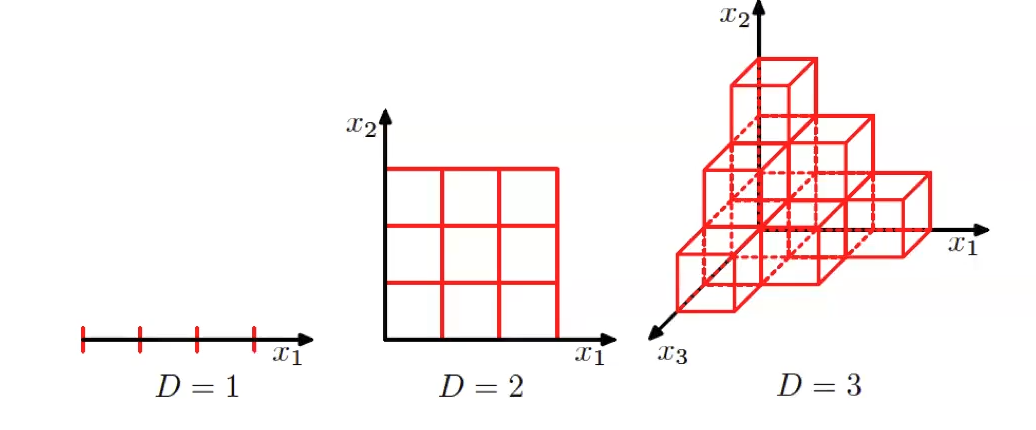
\includegraphics[scale=0.25]{screenshots/2026-03-10_4.png}
		\end{center}
		\begin{itemize}
		    \item The number of cells grows exponentially
		    \item k-NN would then require an exponential growth of the data to cover the entire space
		\end{itemize}
		Handling high-dimensional data also make $k-NN$ memory inefficient, we need to store all the training data to compute distances.
		
		Fortunately, real data often lies in much smaller subspaces, what we means by that is we don't necessarly need to span all space in order to make correct enough guess. Spanning a smaller spaces might be enough. In a few weeks, we will talk about how to find the low dimensional subspace of a given dataset.
	\end{parag}



\subsection{Summary}
\begin{parag}{Advantages}
	\begin{itemize}
	    \item Simple method
	    \item Effective to handle nonlinear data
	    \item Only requires defining one paramter $\left(k\right)$
	\end{itemize}
\end{parag}
\begin{parag}{Drawbacks}
    \begin{itemize}
		\item The results depend on $k$
		\item Becomes expensive as $N$ and/or $D$ grow
		\item May be unreliable with a large $D$
    \end{itemize}
\end{parag}



\section{Nonlinear classification}

The question we will try to answer now is: how can we hadle this data:
\begin{center}
    
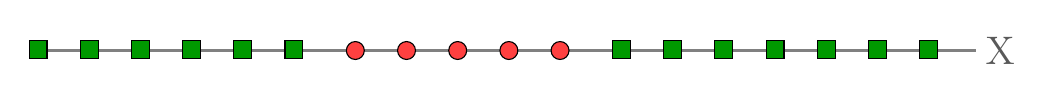
\begin{tikzpicture}[x=0.65cm,y=0.65cm]

    % horizontal axis
    \draw[gray, line width=1pt] (0,0) -- (18.5,0);
    \node[gray!70!black, right] at (18.5,0) {\Large X};

    % green squares on the left
    \foreach \x in {0,1,2,3,4,5}
        \filldraw[fill=green!60!black, draw=black] (\x,-0.15) rectangle ++(0.35,0.35);

    % red circles in the middle
    \foreach \x in {6.2,7.2,8.2,9.2,10.2}
        \filldraw[fill=red!75, draw=black] (\x+0.175,0) circle (0.175);

    % green squares on the right
    \foreach \x in {11.4,12.4,13.4,14.4,15.4,16.4,17.4}
        \filldraw[fill=green!60!black, draw=black] (\x,-0.15) rectangle ++(0.35,0.35);

\end{tikzpicture}

\end{center}
Now what if the red circle here are centered around $0$. Then maybe by transforming our input data we will be able to handle it. Let us create a mapping:
\begin{align*} 
	x \to [x, x^2]
\end{align*}
Then if we mapped this new input:
\begin{center}
	\begin{tikzpicture}[scale=1]

% axes
\draw[gray] (-4.5,0) -- (4.8,0);
\draw[gray] (0,-0.2) -- (0,5);

\node[gray,right] at (4.8,0) {$X$};
\node[gray,above] at (0,5) {$X^2$};

% horizontal line
\draw[blue, thick] (-2.4,0.6) -- (2.8,0.6);

% green squares (points on x^2 outside interval)
\foreach \x in {-3.5,-3,-2.5,-2,-1.5,1.5,2,2.5,3,3.5}{
    \pgfmathsetmacro{\y}{(\x*\x)/3} % scaling factor for nicer figure
    \filldraw[fill=green!60!black,draw=black]
        (\x-0.08,\y-0.08) rectangle (\x+0.08,\y+0.08);
}

% red circles (points on x^2 near minimum)
\foreach \x in {-1,-0.5,0,0.5,1}{
    \pgfmathsetmacro{\y}{(\x*\x)/3}
    \filldraw[fill=red!80,draw=black] (\x,\y) circle (0.11);
}

\end{tikzpicture}
\end{center}
In this new space we can now linearly seperate our data.\\
$ $\\
Now what if our data like this:
\begin{center}
    

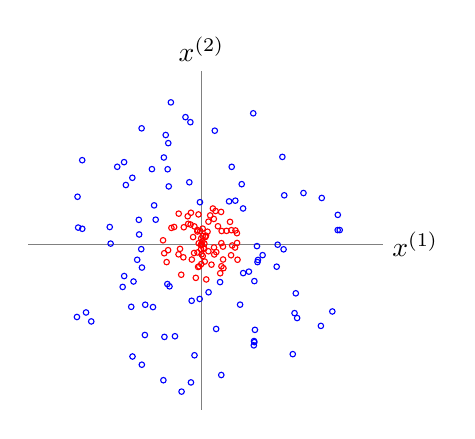
\begin{tikzpicture}

% axes
\draw[gray] (-2.2,0) -- (2.3,0);
\draw[gray] (0,-2.1) -- (0,2.2);

\node[right] at (2.3,0) {$x^{(1)}$};
\node[above] at (0,2.2) {$x^{(2)}$};

% outer blue ring
\foreach \i in {1,...,90}{
    \pgfmathsetmacro{\angle}{360*rand}
    \pgfmathsetmacro{\r}{1.2 + 0.7*rand}
    \filldraw[draw=blue, fill=none] 
        ({\r*cos(\angle)}, {\r*sin(\angle)}) circle (0.035);
}

% inner red cluster
\foreach \i in {1,...,80}{
    \pgfmathsetmacro{\angle}{360*rand}
    \pgfmathsetmacro{\r}{0.5*rand}
    \filldraw[draw=red, fill=none] 
        ({\r*cos(\angle)}, {\r*sin(\angle)}) circle (0.035);
}

\end{tikzpicture}

\end{center}


Intuitively this is the same case as the one before but in 2D, we could create a mapping for instance:
\begin{align*} 
	\begin{pmatrix} x^{\left(1\right)} \\ x^{\left(2\right)} \end{pmatrix}  \to \begin{pmatrix} x^{\left(1\right)} \\ x^{\left(2\right)} \\ \left(x^{\left(1\right)}\right)^2 \end{pmatrix} 
\end{align*}
Which should give the 'same' output as what we have done before. And this is pretty intuitive, we are mapping to the length of the circle as our data was bounded by a circle. And because our boundary is given as a circle, by 'mapping' our data into circle, then the boundary become linear.

\pgfplotsset{compat=1.18}

\begin{center}
    



\begin{tikzpicture}
\begin{axis}[
view={60}{25},
xlabel={$x^{(1)}$},
ylabel={$x^{(2)}$},
zlabel={$x_1^2+x_2^2$},
xmin=-2.2,xmax=2.2,
ymin=-2.2,ymax=2.2,
zmin=0,zmax=4.5,
width=12cm,
height=9cm,
grid=major,
]

% ---- red cluster (center) ----
\addplot3[
only marks,
mark=o,
mark size=1.5pt,
draw=red,
] 
table[row sep=\\]{
x y z
};
\pgfplotsinvokeforeach{1,...,80}{
\pgfmathsetmacro{\angle}{360*rand}
\pgfmathsetmacro{\r}{0.45*rand}
\pgfmathsetmacro{\x}{\r*cos(\angle)}
\pgfmathsetmacro{\y}{\r*sin(\angle)}
\pgfmathsetmacro{\z}{\x*\x+\y*\y}
\addplot3[only marks,mark=o,mark size=1.5pt,draw=red]
coordinates {(\x,\y,\z)};
}

% ---- blue ring (outer class) ----
\pgfplotsinvokeforeach{1,...,120}{
\pgfmathsetmacro{\angle}{360*rand}
\pgfmathsetmacro{\r}{1.5+0.7*rand}
\pgfmathsetmacro{\x}{\r*cos(\angle)}
\pgfmathsetmacro{\y}{\r*sin(\angle)}
\pgfmathsetmacro{\z}{\x*\x+\y*\y}
\addplot3[only marks,mark=o,mark size=1.3pt,draw=blue]
coordinates {(\x,\y,\z)};
}

\end{axis}
\end{tikzpicture}
\end{center}




\subsection{Polynomial curve fitting}

Given that we have training observations (blue circles, 1D input, 1D output) coming from the true green curve:

\begin{center}
\begin{tikzpicture}
\begin{axis}[
    width=11cm,
    height=7cm,
    xmin=0, xmax=1.05,
    ymin=-1.5, ymax=1.5,
    xlabel={$x$},
    ylabel={$y$},
    axis lines=box,
    xtick={0,1},
    ytick={-1,0,1},
]

% smooth green curve
\addplot[
    domain=0:1,
    samples=200,
    thick,
    green!70!black
]
{sin(deg(2*pi*x))};

% data points
\addplot[
    only marks,
    mark=o,
    mark size=2.5pt,
    blue,
]
coordinates{
(0.03,0.35)
(0.14,0.85)
(0.22,1.02)
(0.33,0.98)
(0.44,0.15)
(0.55,0.18)
(0.65,-0.85)
(0.76,-0.45)
(0.87,-0.55)
(1.02,0.25)
};

\end{axis}
\end{tikzpicture}
    
\end{center}


What we can do here is to find a polynomial that approximates the true curve using these observations.\\
$ $\\
Such a polynomial function of degree $M$ can be written as:
\begin{align*} 
	y = w^{\left(0\right)} + w^{\left(1\right)}x + w^{\left(2\right)}x^2 + \cdots + w^{\left(M\right)}x^{M} =  \sum_{j= 0}^{M}w^{\left(j\right)}x^{j}
\end{align*}
Where the $\left\{w^{\left(j\right)}\right\}$ are the coefficients of the different terms, but $x^{j}$ represents $x$ to the power $j$.

\begin{parag}{Polynomial feature expansion}
    In essence, in the three examples, we performed a change of variables:
	\begin{itemize}
	    \item In the first case: $x \to \phi\left(x\right) =  \begin{pmatrix} x & x^2 \end{pmatrix} $
		\item In the second case: $x \to \phi\left(x\right) = \begin{pmatrix} x^{\left(1\right)} \\ x^{\left(2\right)} \\ \left(x^{\left(1\right)}\right)^2 + \left(x^{\left(2\right)}\right)^2 \end{pmatrix} $
		\item In the last (polynomial) case: $x \to \phi\left(x\right) = \begin{pmatrix} 1 \\ x \\ x^2 \\ \vdots \\ x^{M} \end{pmatrix} $
	\end{itemize}
	In general, for $D$-dimensional inputs, we can obtain a large $\phi\left(x\right)$ such that:
	\begin{align*} 
		\phi\left(x\right) = \begin{pmatrix} 1 \\ x^{\left(1\right)} \\ \vdots \\ x^{\left(D\right)} \\ \left(x^{\left(1\right)}\right)^2 \\ \vdots \\ \left(x^{\left(D\right)}\right)^2 \\ \vdots \\ \left(x^{\left(1\right)}\right)^{M} \\ \vdots \\ \left(x^{\left(D\right)}\right)^{M} \\ x^{\left(1\right)}x^{\left(2\right)} \\ \vdots \\ x^{\left(1\right)}x^{\left(D\right)} \\ \vdots \\ x^{\left(D - 1\right)}x^{\left(D\right)} \\ \left(x^{\left(1\right)}\right)^2x^{\left(2\right)} \\ \vdots \end{pmatrix} 
	\end{align*}
	An important thing to understand here is that we are just expanding our input to our usual linear model, nothing more. In essence, polynomial feature expansion uses a mapping from $x \in \mathbb{R}^{D}$ to another representation $\phi\left(x\right) \in \mathbb{R}^{F}$, where $F \gg D$. But we can still use a linear model in this new space and write:
	\begin{align*} 
		\hat{y}_i = w^{T}\phi\left(x_i\right)
	\end{align*}
	Where now $w \in \mathbb{R}^{F}$ (assuming that the 1 accounting for the bias has been incorporated in $\phi$). 
\end{parag}
\begin{parag}{Training expanded features}
    For linear regression, we used the least-square loss:
	\begin{align*} 
		\min_w \sum_{i= 1}^{N}\left(w^{T}x_i - y_i\right)^2
	\end{align*}
	With our expanded features, we can re-write this as:
	\begin{align*} 
		\min_w \sum_{i= 1}^{N}\left(w^{T}\phi\left(x_i\right) - y_i\right)^2
	\end{align*}
	Not that the $w$ vector in the two equations above are different:
	\begin{itemize}
	    \item  In the first, $w \in \mathbb{R}^{D + 1}$
	    \item In the second, $w \in \mathbb{R}^{F}$
	\end{itemize}
	This new function is still convex, and its gradient is given by:
	\begin{align*} \nabla R =  2 \sum_{i= 1}^{N}\phi\left(x_i\right)\left(\phi\left(x_i\right)^{T}w - y_i\right) \end{align*}
	Setting it to zero means that
	\begin{align*} \underbrace{\left(\sum_{i= i}^{N}\phi\left(x_i\right)\phi\left(x_i\right)^{T}\right)}_{F \times F}\underbrace{w^{\ast}}_{F \times 1} =  \underbrace{\sum_{i= 1}^{N}\phi\left(x_i\right)y_i}_{F \times 1} \end{align*}
	We then can group the transformed inputs $\left\{\phi\left(x_i\right)\right\}$ and the output $\left\{y_i\right\}$ in a matrix and vector of the form
	\begin{align*} 
		\Phi = \begin{pmatrix} \phi\left(x_1\right)^{T} \\ \phi\left(x_2\right)^{T} \\ vdd  \\ \phi\left(x_N\right)^{T} \end{pmatrix}  \in \mathbb{R}^{N \times F}\\
		y =  \begin{pmatrix} y_1 \\ y_2 \\ \vdots \\ y_n \end{pmatrix} \in \mathbb{R}^{N}
	\end{align*}
	Then we have:
	\begin{align*} 
		w^{\ast} = \left(\Phi^{T}\Phi\right)^{-1} \Phi^{T}y
	\end{align*}
	
\end{parag}
\begin{parag}{Mapping to a higher-dimensional space}
    In all the examples considered before, the mapping $\phi$ increases the dimensionality of the input to the linear model:
	\begin{itemize}
	    \item From 1 to 2 in the first toy example
	    \item From 2 to 3 in the second one
	    \item From 1 to $M + 1$ in the polynomial fitting case
	\end{itemize}
	
	\begin{center}
	\textbf{But why is higher dimension good?}	
	\end{center}
	Higher dimension give us more \important{flexibility}. There is a theorem called Cover's theorem which said that as you increase the dimension \important{non-linearly}, you increase the probability of making the data linearly seperable.\\
	$ $\\
	None that it is important for the mapping $\phi$ to be \important{nonlinear}. A linear mapping would not result in a nonlinear model in the original space. To show this, let us consider the following linear mapping from a 2D input $x$ to a 3D representation $\phi\left(x\right)$:
	\begin{align*} 
		\begin{pmatrix} x^{\left(1\right)} \\ x^{\left(2\right)} \end{pmatrix}  \to \begin{pmatrix} x^{\left(1\right)} \\ x^{\left(2\right)} \\ x^{\left(1\right)} + x^{\left(2\right)} \end{pmatrix} 
	\end{align*}
	Then, a linear model applied to $\phi$ would have the form:
	\begin{align*} 
		y &=  w^{\left(0\right)} + w^{\left(1\right)}x^{\left(1\right)} + w^{\left(2\right)}x^{\left(2\right)} + w^{\left(3\right)}\left(x^{\left(1\right)} + x^{\left(2\right)}\right)\\
		  &= w^{\left(0\right)} + \left(w^{\left(1\right)} + w^{\left(3\right)}\right)x^{\left(1\right)} + \left(w^{\left(2\right)} + w^{\left(3\right)}\right)x^{\left(2\right)}
	\end{align*}
	Which is equivalent to:
	\begin{align*} 
		y = w^{\left(0\right)} + \overline{w}^{\left(1\right)}x^{\left(1\right)} + \overline{w}^{\left(2\right)}x^{\left(2\right)}
	\end{align*}
	Which implies that there is no nonlinear behavior.
	
\end{parag}









